\chapter{User Guide}
\label{ch:user_guide}


In the previous chapter we developed and evaluated several methods for a known-item-search task. In this chapter we provide a user guide for our implementation of aforementioned solutions. This chapter only covers user interaction and does not cover creating new datasets nor starting the server. For the latter check the Programmer's Guide chapter \ref{ch:developers_guide}

The user can access the application via web-based interface. Once the webpage is opened we can see by default a module for spatial similarity search (refer to \ref{ch:TODO}). \todo{} The second module includes face similarity search (chapter \ref{ch:face_search}). We describe both modules in the same order.

\section{Spatial Similarity}

On the screen we can see a canvas for creating the queries and some control elements. On the first load, a query image (the searched scene) is displayed for several seconds over the canvas. During the creation of the collage we can always access the query image by clicking on the image button. The number of hints, i.e., how many times was query shown, is logged. 



\subsection*{Creating a query}

We can create custom queries in the canvas. In order to add an image to the canvas, we can either paste it, or add it based on the url of the image. To paste an image, it needs to be available in the clipboard. The easiest way to do that for most images is to right click on the image and select "Copy image". We can also recommend a selective screenshot features, which can speed up the copying of the images and also adds a possibility for selecting only a part of the image. For Windows 10 it is possible via key combination Shift + Win Key + S. There is no limitation on the number of images in the collage, although the increased number may reduce the performance (as they may be misleading hints) in recall and also it prolongates the computation time needed for the query to process.

Once the image is placed in the canvas, we can resize it by grabbing bottom right corner, or move it by dragging. To remove the image click on the X button in the top right corner. To query the model, click the "Query" button. By default, automatic querying is turned off, i.e., after each movement or resizing the system automatically queries for new results. This can be turned off, especially in case of more computationally heavy models.

The user interface also provides easy switch between the approach used (as described in the chapters \ref{ch:TODO} and \ref{ch:TODO}). \todo{} This can be accessed by clicking on the dost, right to the "Query" button. 

\subsection*{Results}

\begin{figure}
    \centering
    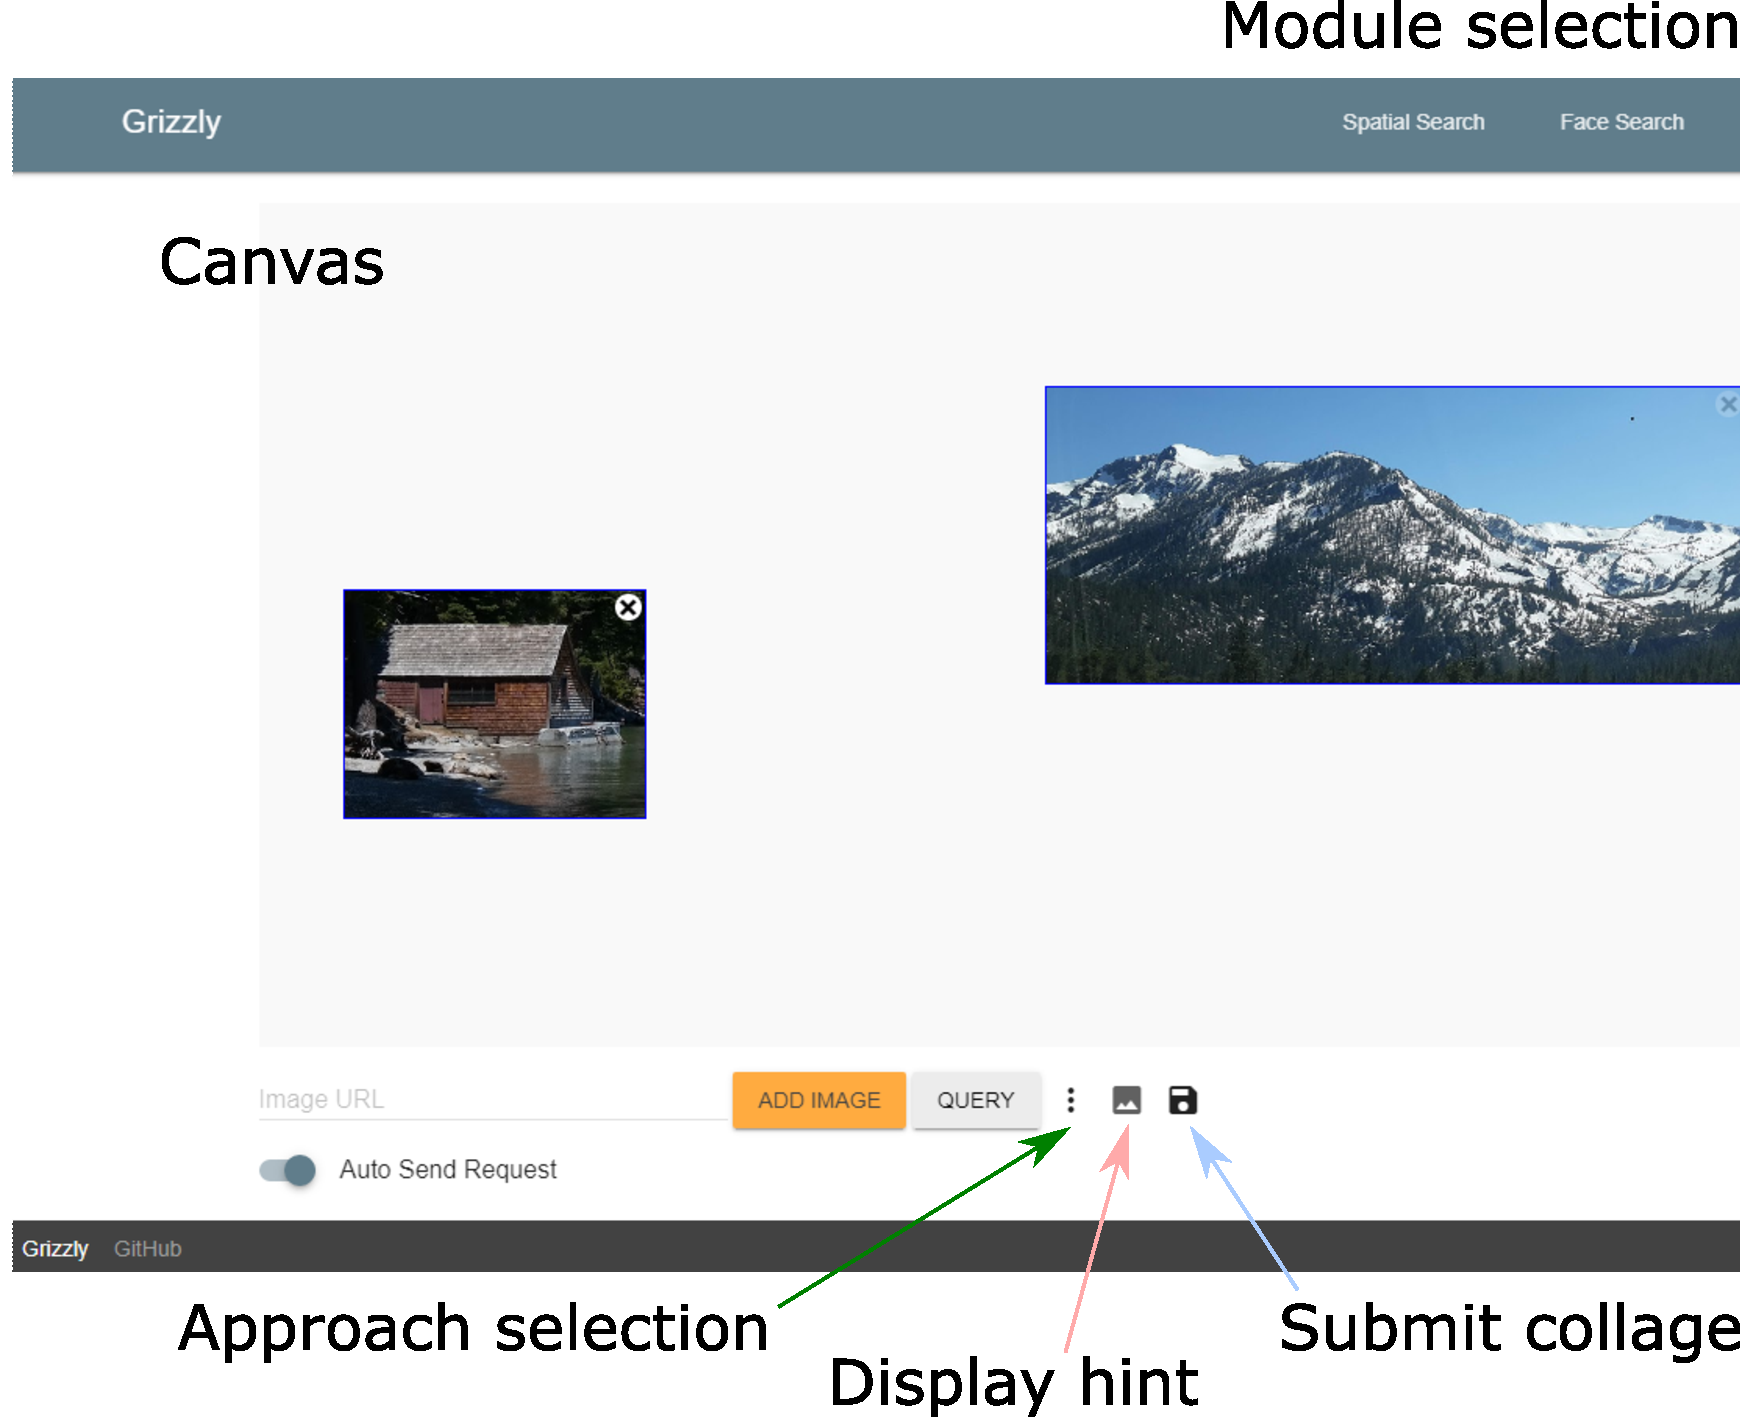
\includegraphics[width=\linewidth]{img/spatial_ui.pdf}
    \caption{User interface for creating collages}
    \label{fig:ui_collage}
\end{figure}

By default, the application displays only the best 100 matched results. The images are reloaded after each successful query. The top of the Results section also displays the rank of the searched item. This helps for the user to learn how to use the tool more effectively. The winning regions are highlighted as well for the regions search.

\section{Face Search}

On the load \todo{During loading time alebo Upon loading the application}, there is a grid with faces and also a query image displayed. Same as in the spatial similarity module, the query image can be accessed at any moment by clicking on the image icon. The face search consists of several layers, where the bottom are the largest and the top the smallest. The user starts on the top layer. Then they can click to step down to the next layer. In the layer they can move within the layer using the navigation buttons at the top of the page. \todo{TODO} button steps up a layer.

Each of the faces also provides a separate way to search. There are two buttons available at the top right corner of all of the faces: video images and face button. Video images button displays all the frames from the same video as the face was retrieved from. The face button returns frames from whole datasets, which contain faces most similar to the one clicked at.

\chapter{Developer's guide}
\label{ch:developers_guide}

\cite{pedregosa2011scikit}
\cite{van2011numpy}

\section{Running the server}

\section{Creating new datasets}



\chapter{Code Structure (programmer's guide)}
\label{ch:programmers_guide}


